\section{Internet und IP-Adressen}

\begin{defi}{Internet}
    Das Internet, ist ein weltweiter Verbund von Rechnernetzwerken, den autonomen Systemen.
    Router werden als koppelnde Elemente zwischen den Teilnetzen genutzt.
\end{defi}

\begin{defi}{Netzwerk (ISO/OSI)}
    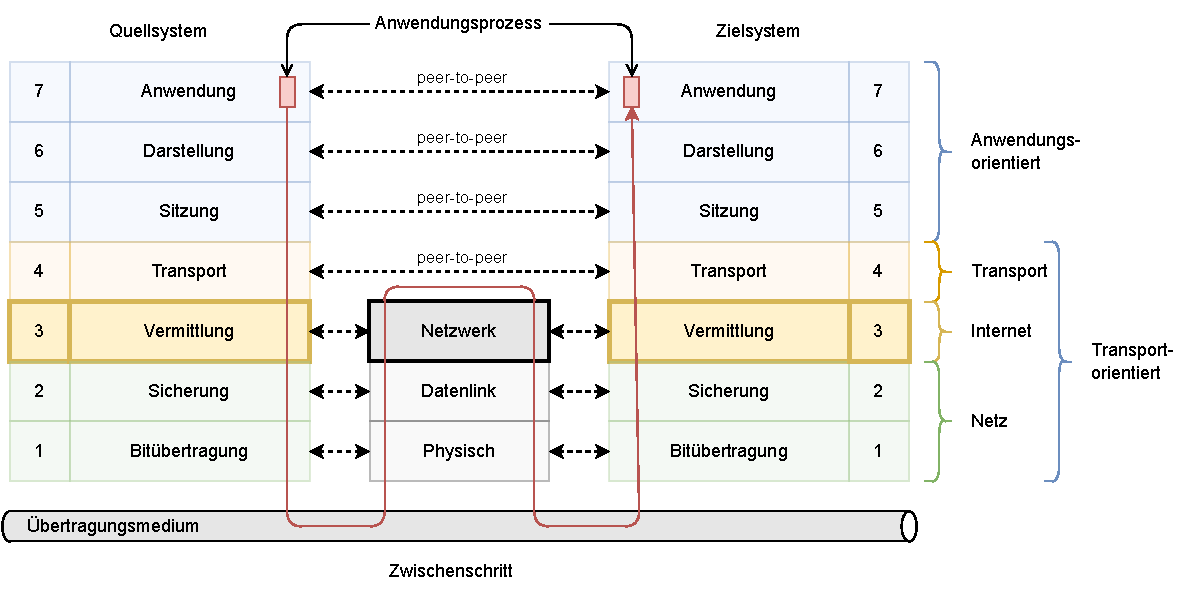
\includegraphics[width=\textwidth]{includes/figures/defi_iso_osi_network.pdf}
\end{defi}

\begin{defi}{TCP/IP}
    \emph{TCP/IP} ist eine protokollunabhängige Ausmodellierung des konzeptionellen \emph{ISO/OSI} Modells.

    \begin{center}
        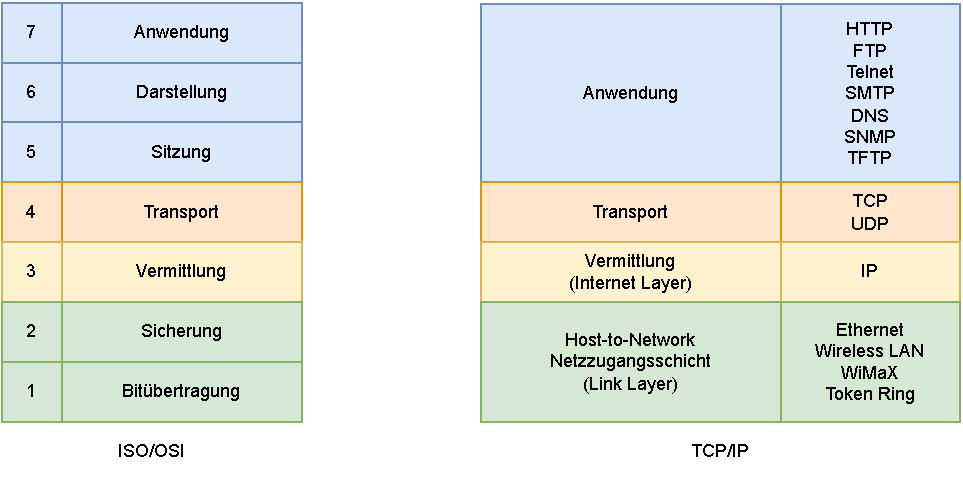
\includegraphics[width=0.75\textwidth]{includes/figures/defi_tcp_ip.pdf}
    \end{center}
\end{defi}

\begin{bonus}{Aufbau des Internets}
    Die Basis des Internets bilden \emph{Tier-1} Internet Service Provider (ISPs).
    Diese treten gleichberechtigt untereinander auf und sind durch vertraglich regulierte Verbindungen angebunden.

    Als Verbindung zwischen den ISPs dienen \emph{Network Access Points} (NAPs) oder \emph{Internet Exchange Points} (IXPs)

    \begin{center}
        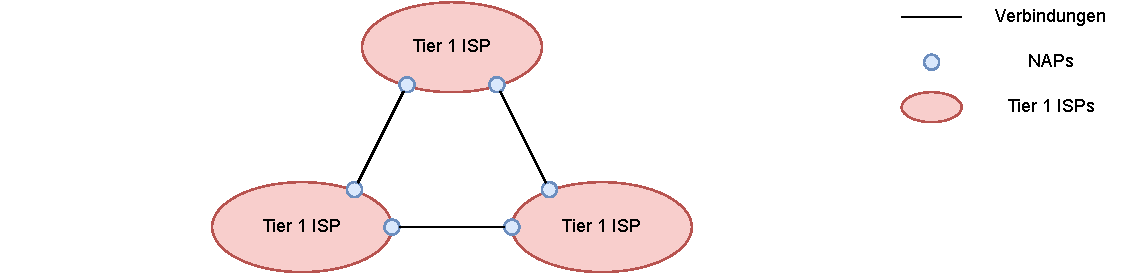
\includegraphics[width=0.75\textwidth]{includes/figures/bonus_aufbau_internet_1.pdf}
    \end{center}
\end{bonus}

\begin{bonus}{Aufbau des Internets}
    \emph{Tier 2} ISPs sind national bzw. regional und sind immer an einen oder mehrere \emph{Tier 1} ISPs angeschlossen.

    Sie treten dabei gegenüber \emph{Tier 1} ISPs als KundIn auf.

    \begin{center}
        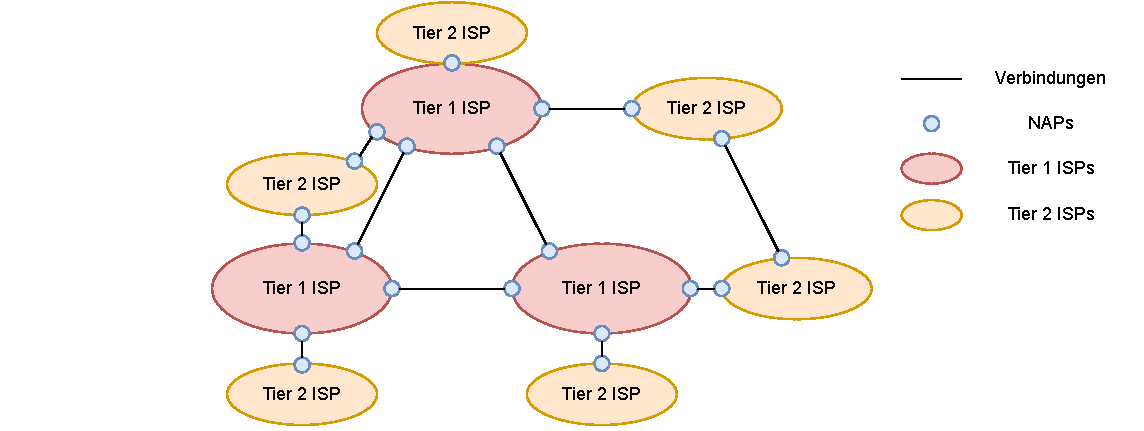
\includegraphics[width=0.75\textwidth]{includes/figures/bonus_aufbau_internet_2.pdf}
    \end{center}
\end{bonus}

\begin{bonus}{Aufbau des Internets}
    \emph{Tier 3} ISPs binden den Kunden beispielsweise über DSL direkt an das gesamte Netzwerk an.

    Sie treten dabei gegenüber \emph{Tier 2} ISPs selber als KundIn auf.

    \begin{center}
        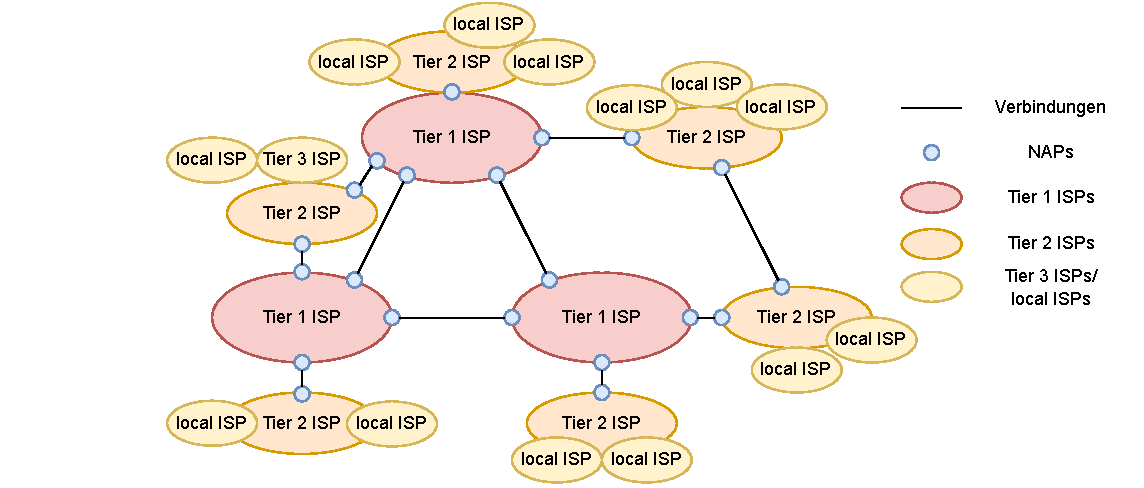
\includegraphics[width=0.75\textwidth]{includes/figures/bonus_aufbau_internet_3.pdf}
    \end{center}
\end{bonus}

\begin{bonus}{Aufbau des Internets}
    \begin{center}
        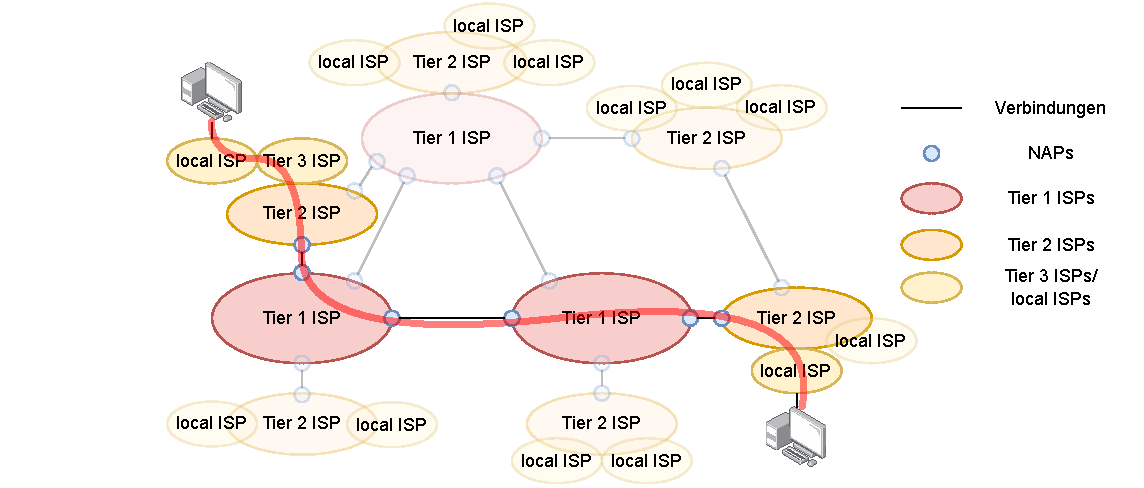
\includegraphics[width=0.75\textwidth]{includes/figures/bonus_aufbau_internet_4.pdf}
    \end{center}
\end{bonus}

\begin{bonus}{Nachrichtenzustellung}
    \begin{wrapfigure}{r}{0.25\textwidth}
        \begin{center}
            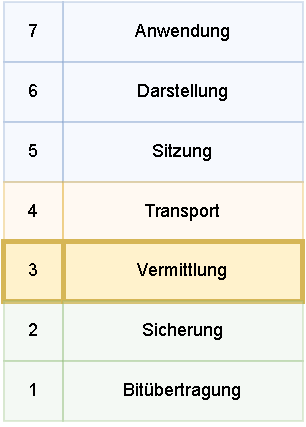
\includegraphics[width=0.2\textwidth]{includes/figures/bonus_iso_osi_vermittlung.pdf}
        \end{center}
    \end{wrapfigure}
    %
    Die Herausforderung in diesem großen Netz aus Netzen ist es Datenpakete von einem beliebigen Endgerät zu einem bestimmten Ziel zu versenden.

    Damit dies gelingt, wird in der Vermittlungsschicht einer der möglichen Wege zum Zielgerät gewählt.
    Die Wegwahl findet durch \emph{Routing Protokolle} statt.

    Die Entscheidung erfolgt durch \emph{Routing Tabellen}.
    In diesen lassen sich - je nach Protokoll - definierte Wege finden, unter denen man das autonome System des Zielgeräts findet bzw. welcher Weg befolgt werden soll, wenn das Zielgerät komplett unbekannt ist.

    In der Vermittlungsschicht wird größtenteils das IP-Protokoll genutzt, um die Pakete zu adressieren und Regeln zur Paketbehandlung aufzustellen.
\end{bonus}

\begin{defi}{Das Internet-Protokoll (IP)}
    \emph{IP} bietet eine Ende-zu-Ende Kommunikation zwischen Endgeräten im Internet.
    Derzeit wird flächendeckend \emph{IPv4} bzw. \emph{IPv6} eingesetzt.

    IP ist paketvermittelnd, leitet also in sich geschlossene, unabhängige Dateneinheiten bzw. Datagramme ungesichert zwischen zwei Endpunkten weiter.
    Jedes Paket wird dabei in dem jeweiligen Router zwischengespeichert, überprüft und dementsprechend aussortiert oder weitergeleitet.
    Da die Pakete parallel von den Routern abgearbeitet werden, kann es passieren, dass:
    \begin{itemize}
        \item Datagramme verloren gehen
        \item Datagramme sich gegenseitig überholen
        \item Datagramme mehrfach ankommen
    \end{itemize}

    \emph{Sitzungen} werden durch einen exklusiven Kommunikationskanal über TCP simuliert.
\end{defi}